\lab{Complex Integration}{Integration in the Complex Plane}{Integration in the Complex Plane}

\objective{Understand the basics of integration in the complex plane}

\section*{Contour Integrals in the Complex Plane}

From multivariable calculus, you may recall that an integral may be taken along a path. This is very similar to what we can be done in the complex plane. Consider the function $f(z)$ on the complex plane. Let $z=x+iy$ Let $u$ and $v$ be the real and imaginary parts of $f$ respectively. We integrate $f$ along some contour $C$ in the complex plane, beginning at $z=a$ and ending at $z=b$. This integral may be written $$\int_c f(z)dz$$ 
Parameterizing $z$, we have $$\int_a^b z(t)z'(t)dt=$$
Expanding into real and imaginary parts, we have
$$\int_a^b (u(z(t))x'(t)-v(z(t))y'(t))dt +i \int_a^b(v(z(t))x'(t)+u(z(t))y'(t))dt$$
We have now written this complex integral as the sum of two real valued integrals in $\mathbb{R}$. Note that this implies that $\int_C z dz$ may depend on the contour we choose and not just on the endpoints $a$ and $b$.

\begin{problem}
Write a function which takes a complex function $f(z)$, a contour parameterization $z(t)$ of a contour $c$, the integration bounds on $t$, and a tolerance and returns the integral of $f$ along the contour $c$. 
You may use the numerical differentiation and integration functions that you have defined in previous labs, or you can use the function \li{mpmath.diff} as the numerical derivative and \li{mpmath.quad} or \li{scipy.integrate.quad} as the numerical integral. (Mpmath is another numerical library you can install. It is used primarily for arbitrary precision computation.)
\end {problem}

\begin{problem}
Using the function you just defined, integrate the following functions along the following contours
\begin{itemize}
\item $e^z$ counterclockwise along the unit ball starting and ending at $1$
\item $\bar{z}$ counterclockwise along the unit ball starting and ending at $1$
\item $e^z$ along a straight line from $0$ to $1+i$
\item $\bar{z}$ along a straight line from $0$ to $1+i$
\item $e^z$ along the real axis from $0$ to $1$, then along the line from $1$ to $1+i$
\item $\bar{z}$ along the real axis from $0$ to $1$, then along the line from $1$ to $1+i$
\item $e^z$ along the unit ball centered at $i$ from $0$ to $1+i$
\item $\bar{z}$ along the unit ball centered at $i$ from $0$ to $1+i$
\end{itemize}
\end{problem}

\begin{problem}
Implement another version of the function from problem $1$ using symbolic differentiation and integration from SymPy. Instead of using callable functions for the function and the contour, use SymPy symbolic expressions. You will have to add parameters for the variables of the expressions for the function and contour. The tolerance parameter should no longer be necessary.
\end{problem}

An important theorem in Complex Analysis is Cauchy's Integral Theorem, which says that, for any holomorphic function on a simply connected  $f(z)$, and two contours $C_1$ and $C_2$ that share endpoints, $$\int_{C_1}f(z)dz = \int_{C_2}f(z)dz$$

Note: A simply connected domain is, roughly speaking, a domain which contains no ``holes." For example, the unit ball is a simply connected domain, while the set $\setconstruct{z\in \mathbb{C}}{1<\abs{z}<2}$ is not. 

In other words, for a holomorphic function on a simply connected domain, the integrals from one point to another are not path dependent for any contours that lie within D.
An immediate consequence of the theorem is that for a complex function $f$, holomorphic on a simply connected domain $D$, and a contour $C$ lying entirely within $D$ which begins and ends at some point $a\in D$, $$\int_C f(z)dz=0$$
An example would be the function $e^z$ which is holomorphic everywhere on the complex plane (when this is true, we say that the function is ``entire"). As a consequence of Cauchy's Integral Theorem, for any two points $a,b\in \mathbb{C}$ , the integral from $a$ to $b$ is path independent.

Cauchy's Integral Theorem allows us to define the antiderivative of a function on a simply connected domain as follows
\begin{theorem}[Cauchy's Integral Theorem]
Let $D$ be a simply connected domain in $\mathbb{C}$. Let $f$ be a function that is holomorphic on $D$. Let $z_0$ and $z$ be points of $D$. Define the antiderivative, $F(z)$, as $\int_C f(z)dz$ for any $C$ in $D$ from $z_0$ to $z$.
\end{theorem}
Given the conditions above, this also lets us evaluate integrals as we would normally do in the real numbers, so we may write $\int_a^b f(z)dz=F(b)-F(a)$ where $F$ is the antiderivative of $f$. It can be proven that that $F$ is also analytic on $D$. It follows that a function which is holomorphic on a domain $D$ is infinitely integrable on that domain.

The quadrature algorithms used in many of the integration algorithms work along a straight line between the integration bounds in the complex plane, so for holomorphic functions we should be able to use the integration function we wrote earlier. The \li{mpmath.quad} function also allows us to do this. For example, integrating $e^z$ from $-1-i$ to $1+i$ can be done numerically as follows.
\begin{lstlisting}[style=python]
import mpmath as mp
complex(mp.quad(lambda x: mp.exp(x),(complex(-1,-1),complex(1,1))))
\end{lstlisting}
In the same case, we can also evaluate this integral using SymPy as follows.
\begin{lstlisting}[style=python]
import sympy as sy
sy.N(sy.integrate(sy.exp(z),(z,-1-sy.I,1+sy.I)))
\end{lstlisting}

\section*{The Cauchy Integral Formula}

Another major theorem in complex analysis is called Cauchy's Integral Formula (not to be confused with Cauchy's Integral Theorem). It states that for a domain $D$ in the complex plane, containing some contour (rigorously speaking, a piecewise Jordan Curve) $C$ and the interior of $C$, for any $z_0$ in the interior of $C$, 
$$f(z_0)=\frac{1}{2\pi i} \int_C \frac{f(z)}{z-z_0} dz$$. 

With more work, this theorem can be used to show that any function $f$ holomorphic on some domain $D$ is also infinitely differentiable on that domain.
In fact the $n$th derivative of $f$ is given by the formula $$f^{(n)}(z_0) = \frac{n!}{2\pi i} \int_C \frac{f(z)}{(z-z_0)^{n+1}} dz$$
This result is also important because it allows us to relate the value of $f$ on the inside of a contour to the value of $f$ on the contour itself. In other words, the values of $f$ inside the contour depend only on the values of $f$ along the contour itself.
A related theorem (the Morera theorem) states that if some function $f$ is continuous on a domain $D$ and for every contour beginning and ending at the same point (properly speaking, a piecewise smooth closed curve), the formula $\int_C f(z) dz = 0$ holds, then $f$ is holomorphic on $D$. 

\begin{problem}
Using Cauchy's Integral Formula, write a python function which returns a callable function which evaluates a complex function $f$ along the interior of a contour $C$. It should accept a callable function for the paramaterization of $C$, a callable function for the values of $f$ along $C$, and the bounds on the parameter used. Note that $C$ must begin and end at the same point and that $f$ must also begin and end with the same value so that $f$ is continuous along $C$.
\end{problem}

Notice that in Cauchy's Integral Formula, we are integrating along a contour that begins and ends at the same point. The function is also holomorphic at every point except $z_0$. At $z_0$ the integrand is undefined and has a singularity. This integral around a singularity has some useful properties.

\section*{Residues}

We will now introduce another form of series representation of functions. A Laurent series of a function is a series of the form $$\sum_{n= -\infty}^{\infty} a_n (z-z_0)^n$$
It can be proven that 
$$a_n = \frac{1}{2\pi i} \int_C \frac{f(z)}{(z-z_0)^{n+1}} dz$$ 
It can also be proven that this series representation is unique.
This sort of series can be generated whether or not $f$ has a singular point a $z_0$. When $f$ does not have a singularity at $z_0$ this representation degenerates to a normal Taylor Series (with the derivatives evaluated by the formula for the $n$th derivative of an analytic function). 
Where $C$ is a contour which passes counterclockwise around the singularity exactly once.
This is called Laurent's Theorem.
By analyzing the convergence of this series, we see that it will either converge for all points except possibly $z_0$ in the complex plane, converge on an annulus about $z_0$, or not converge at all.

\begin{problem}
Write a python function which takes $f$, $z_0$, the lowest power term in the Laurent Series, and the highest power term in the Laurent Series and returns a callable function for the desired series.
\end{problem}

The built in function \li{sympy.series} can also evaluate the series expansion of a function at a singularity, for example
\begin{lstlisting}[style=python]
import sympy as sy
import sympy as sy
(1/sy.sin(z)).series(z,0,8)
\end{lstlisting}
which evaluates the series expansion of the $\csc(z)$ at $z=0$. 
As is the case with Taylor Series, often the Laurent Series expansion of a function is not computed directly using it's integral definition. It is, rather, obtained by substitution into known series. For example, 
$$e^z = \sum_{n=0}^{\infty} \frac{z^n}{n!}$$, so we may say,
$$e^{1/z} = \sum_{n=0}^{\infty} \frac{1}{n! z^n}$$

\begin{problem}
Find the Laurent Series expansion of the function $\frac{e^{z}}{z^2 +1}$
\end{problem}

%%% Before final publication we should figure out how to get the z=z_0 underneath the symbol Res. For now I'll just leave
%%% it alone. A class can be done off of this as it is written.

The term corresponding to $n=-1$ in the Laurent Series expansion of a complex function $f$ about a singularity $z_0$ is called the residue of $f$ at $z_0$ and is often written $\Res_{z=z_0} f(z)$.
From Laurent's Theorem, using $f$, $z_0$, and $C$ as defined above, we have that $$Res_{z=z_0} f(z) = \frac{1}{2 \pi i} \int_C f(z) dz$$.
Another major theorem in Complex Analysis is the residue theorem (Also called Cauchy's Residue Theorem) which states that for some contour $C$ which does not intersect itself and a function $f$ analytic on $C$ and on the interior of $C$ except for isolated singular points $z_1,...,z_n$, that 
$$\int_C f(z) dz = 2 \pi i \sum_{k=1}^{n} \Res_{z=z_k} f(z)$$
This allows for the evaluation of integrals that might not be pleasant in other circumstances.
%% Maybe an example would be nice here... idk. That'll mostly be in the next lab though.
Here are a few definitions that are good to know when speaking of residues.
\begin{itemize}
\item A singular point $z_0$ is said to be an ``isolated singular point" of a function $f$ if no sequence of singular points of $f$ converges to it.
\item An isolated singular point $z_0$ is said to be a removable singular point of a function $f$ if there are no negative powers of $(z-z_0)$ in the Laurent series expansion of $f$.
\item An isolated singular point $z_0$ is said to be a pole of a function $f$ is there are finitely may terms containing negative powers of $(z-z_0)$ in the Laurent series expansion of $f$. 
\item An isolated singular point $z_0$ is said to be an essential singular point of a function $f$ if there are infinitely many negative powers of $(z-z_0)$ in the Laurent series expansion of $f$.
\end{itemize}

\begin{problem}
Evaluate the residue of $\sin(\frac{1}{z})$ at $z=0$ by substituting into known Taylor series expansions. Check your result numerically.
\end{problem}

\begin{problem}
There is a direct relationship between the partial fraction decomposition of the reciprocal of a polynomial and the residues of that function at its zeroes. Show why this is true, and, using the Newton's method function you have already written, write a function which, given the coefficients for a polynomial, returns the coefficients for the partial fraction decomposition of its reciprocal with the zeroes corresponding to each coefficient.
\end{problem}
 
\section*{Multi-Valued Functions}

Another important topic in Complex Analysis is the study of multiple valued functions. These functions arise as we consider the inverses of functions that are not strictly one to one on the complex plane. A classic example is $\sqrt{x}$. Which may take two values for every nonzero point of the complex plane.

In the Real numbers we worked with functions like this by simply restricting their output on a certain domain. We can do a similar thing in the Complex plane. Loosely speaking, such a restriction is called a branch. The function $\sqrt{z}$ has two branches on the complex plane. We cut it along the ray $(0,-\infty)$. By doing so, we can define two single valued functions on the complex plane. We call inverse functions that have multiple values like this ``multi-valued functions" or ``multifuctions." Computationally we restrict the output to a single portion of the actual possible values of the multifunction. We can still visualize the ``Riemann surfaces" of multifunctions in the complex plane. The following are some simple examples.
\begin{figure}[h]
\begin{subfigure}{.49\textwidth}
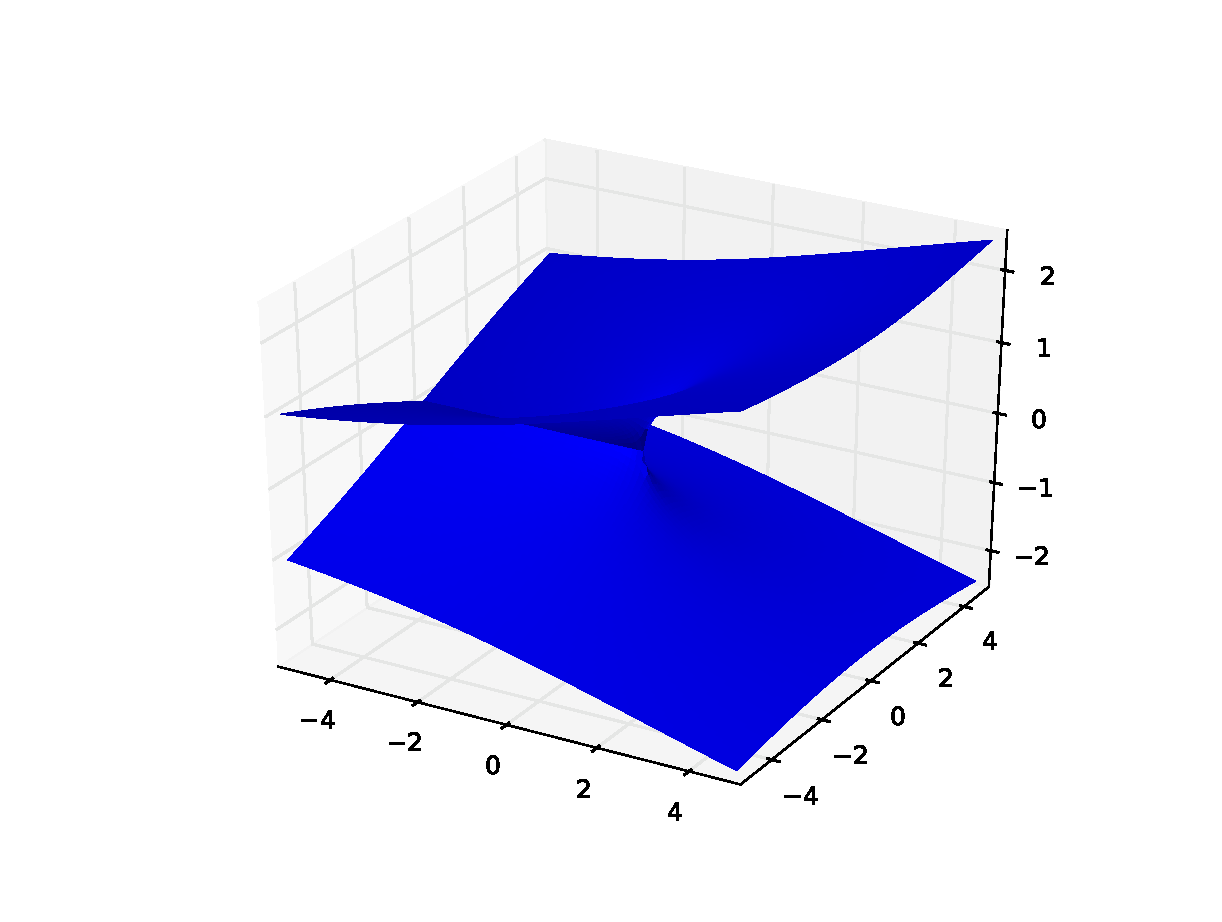
\includegraphics[width=\textwidth]{RiemannSurface1}
\caption{The Real Part of $\sqrt{z}$}
\end{subfigure}
\begin{subfigure}{.49\textwidth}
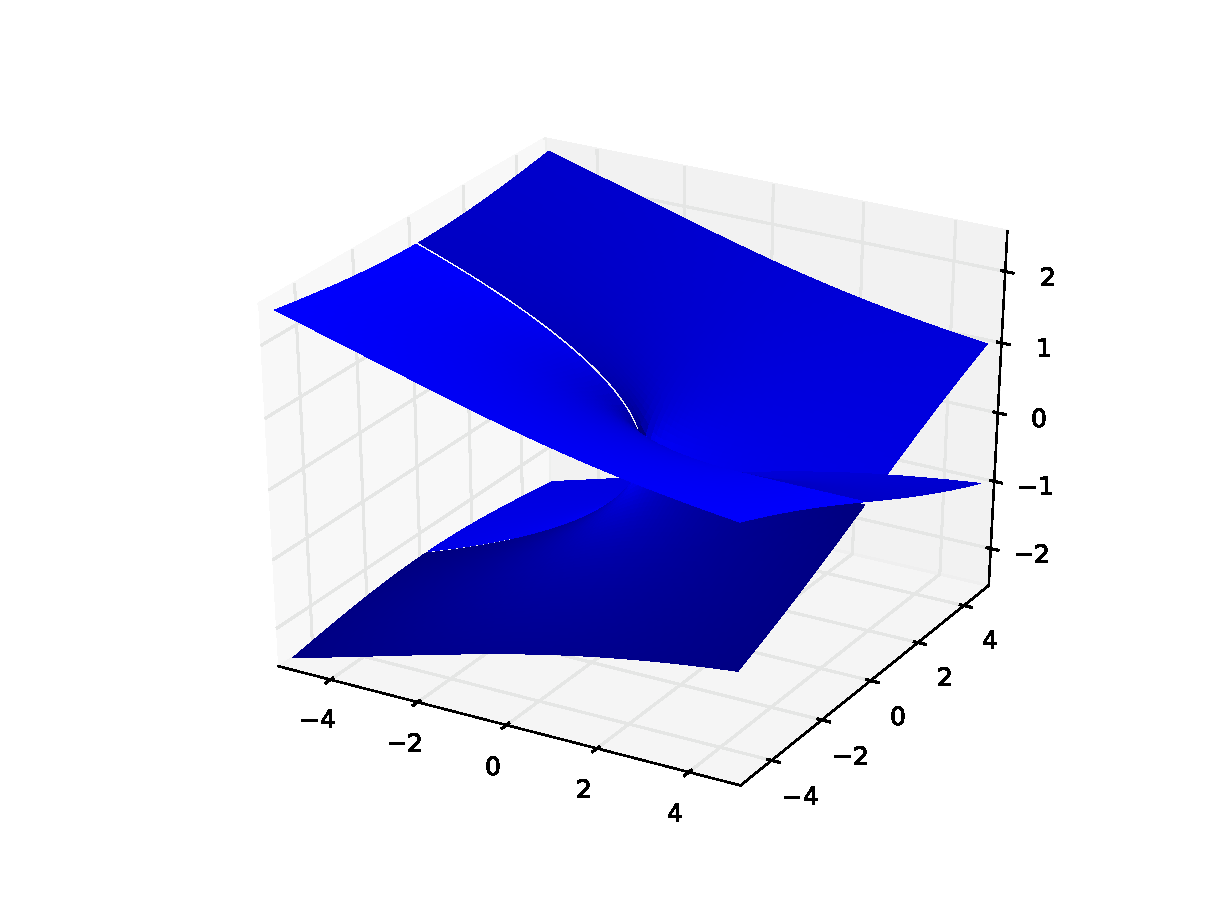
\includegraphics[width=\textwidth]{RiemannSurface2}
\caption{The imaginary part of $\sqrt{z}$}
\end{subfigure}
\end{figure}
These are some very basic examples. Riemann surfaces can be very complex. Another simple example is $\ln(z)$ which has a single value for the real part, and the following for its imaginary part:
\begin{figure}[h]
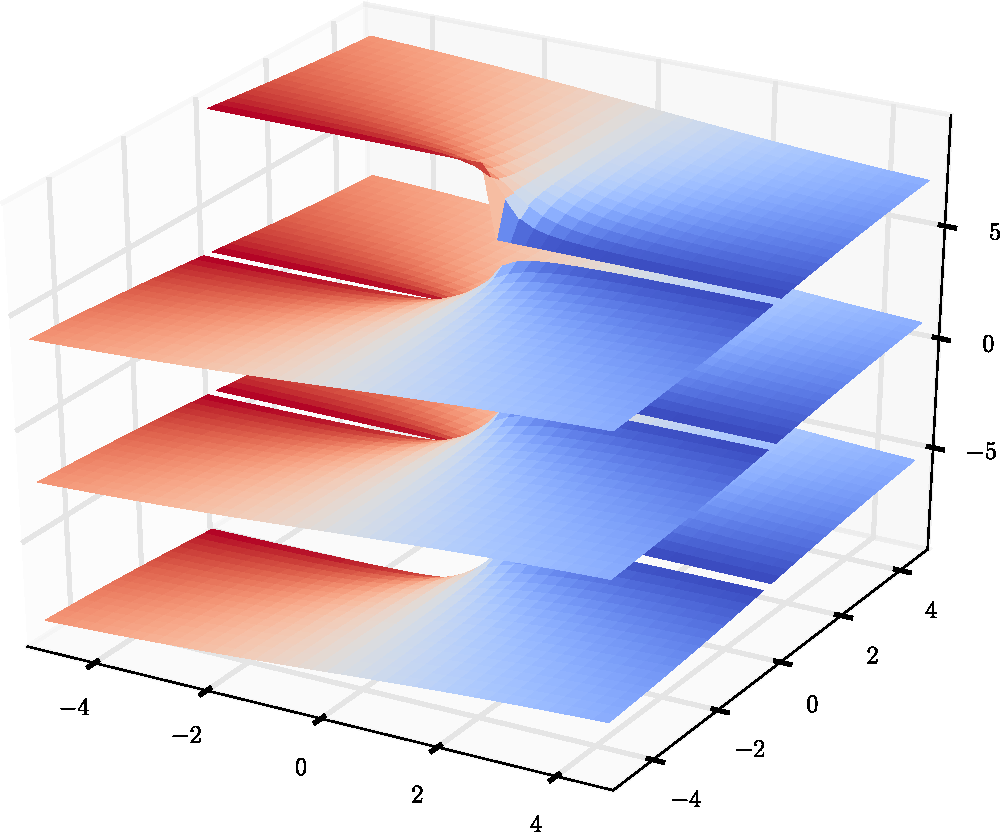
\includegraphics[width=\textwidth]{RiemannSurface3}
\caption{Riemann surface plot of $\ln(z)$}
\end{figure}
Note that this is only a portion of the Riemann surface of $\ln(z)$. The full surface is, in actuality, an infinite spiral that repeats every $2\pi$. This is because for any complex $z\neq 0$, we have $e^z=e^{z+2n\pi}$ where $n$ is any integer.
\begin{figure}[h]
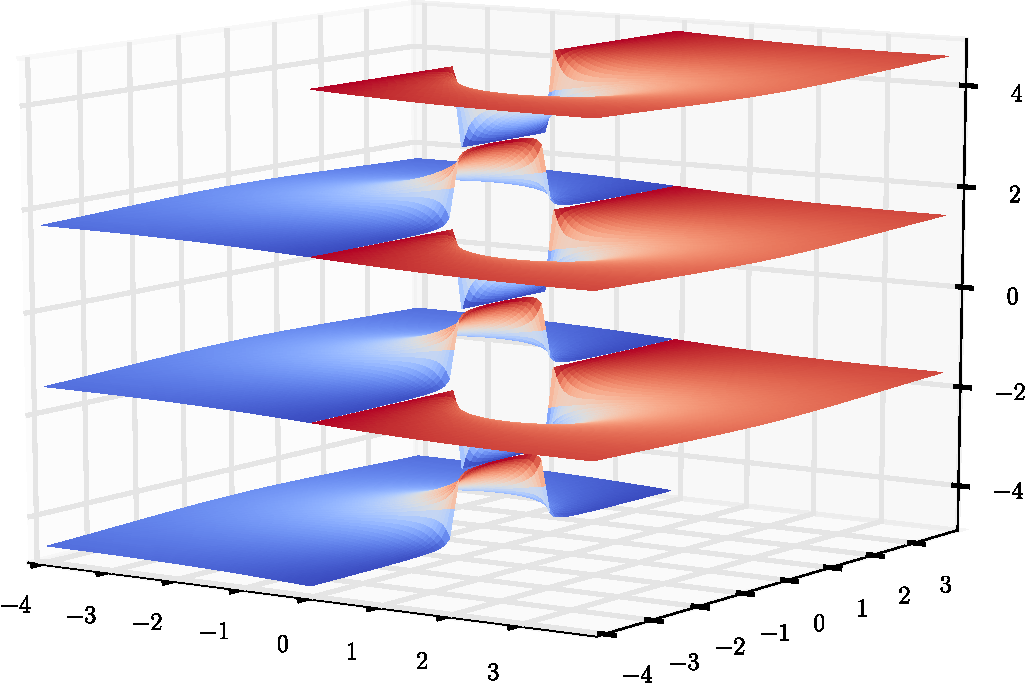
\includegraphics[width=\textwidth]{RiemannSurface4.pdf}
\caption{Even the Riemann surface of $\arctan(z)$ becomes increasingly complex. This is a graph of a portion of the Riemann surface for the real part of $\arctan(z)$.}
\end{figure}
All three of the functions we have plotted can be made analytic at almost any point, except at their singularities, but that depends on how we cut the domain to give it a single value. When Integrating such functions be careful about integrating across such cuts in the domain.

\begin{problem}
Plot the Riemann surface of $z^{\frac{1}{4}}$.
\end{problem}

\begin{problem}
Integrate the function $\ln(z)$ beginning at $z=1$ and $\ln(z)=0$ and ending at $z=1$ and $\ln(z)=6*\pi$.
\end{problem}